\subsection{MFCC Computation}

\begin{frame}[allowframebreaks]{MFCCs: Intuition \& Practice}

\begin{itemize}
    \item Mel-Frequency Cepstral Coefficients (MFCCs) provide a compact summary of the log-Mel spectrum, obtained by decorrelating features with a Discrete Cosine Transform (DCT).  
    \item This representation captures the \textbf{spectral envelope} (linked to vocal-tract shape) while discarding fine pitch details.  
    
    \item Typical processing pipeline:
    \begin{itemize}
        \item (Optional) pre-emphasis to boost high frequencies.
        \item Frame the signal, apply a window, and compute the STFT.
        \item Apply a mel filterbank to obtain band energies.
        \item Take logarithms of the energies.
        \item Apply DCT to decorrelate; keep the first $Q$ coefficients (e.g., 13).
        \item Optionally append temporal derivatives ($\Delta$) to capture dynamics.
    \end{itemize}
\framebreak
    \item Why MFCCs are important:
    \begin{itemize}
        \item Historically very strong for HMM-GMM based ASR systems.
        \item Emphasize formant structure and vocal-tract characteristics.
        \item Tend to suppress pitch information, which is often less useful for recognition tasks.
    \end{itemize}
\end{itemize}

\end{frame}


\begin{frame}[fragile,allowframebreaks]{MFCC Computation}
    \begin{itemize}
    \item MFCCs are widely used in speech and audio processing.
    \item They capture the timbral texture of audio signals.
    \item Typically, only the first 13 coefficients are used for feature extraction.
\end{itemize}
\framebreak
\begin{figure}
    \centering
    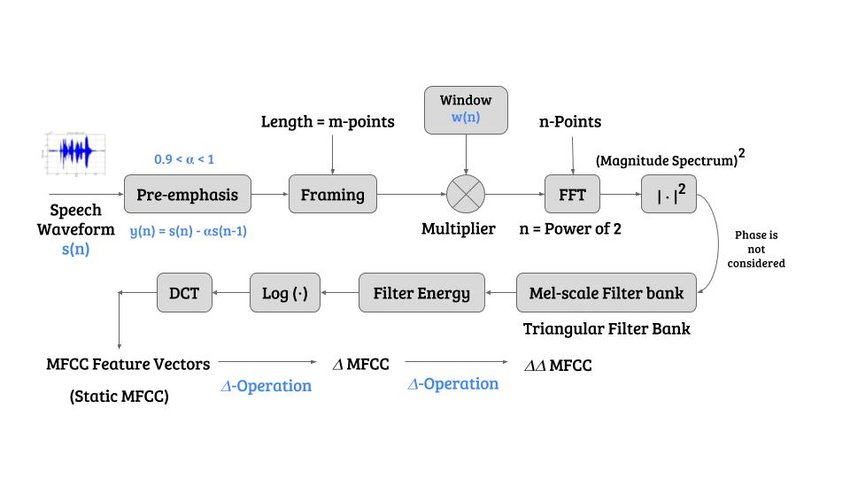
\includegraphics[width=1.08\textwidth,height=0.8\textheight,keepaspectratio]{images/audio-nlp/mfcc.png}
    \caption*{A block diagram for MFCC computation: From audio signal to MFCC features.}
\end{figure}
\framebreak
\textbf{Pipeline:}
\begin{enumerate}
    \item Compute log-Mel spectrogram
    \item Apply Discrete Cosine Transform (DCT)
    \item Keep first 13 coefficients (MFCCs)
\end{enumerate}

\textbf{MFCC Equation:}
\begin{equation}
    c_k = \sum_{n=1}^{N} \log(E_n) \cos\left[ \frac{\pi k}{N} \left( n - \frac{1}{2} \right) \right]
\end{equation}
where:
\begin{itemize}
    \item $c_k$ is the $k$-th MFCC coefficient
    \item $E_n$ is the energy in the $n$-th Mel filter
    \item $N$ is the total number of Mel filters
\end{itemize}
\end{frame}

\begin{frame}[allowframebreaks]{MFCC Math (Lightweight but Concrete)}

\begin{itemize}
    \item MFCCs are built from three main mathematical steps:
    \begin{enumerate}
        \item \textbf{Band energies (Mel filtering):}
        \[
            E_m = \sum_{k} |X[k]|^2 \, H_m[k]
        \]
        where $H_m$ is the $m$-th triangular Mel filter.
        
        \item \textbf{Logarithmic compression:}
        \[
            L_m = \log(E_m + \epsilon)
        \]
        which stabilizes values and mimics loudness perception.
        
        \item \textbf{DCT-II (decorrelation):}
        \[
            c_q = \sum_{m=1}^{M} L_m \cos\!\left[\frac{\pi q}{M}\,(m - \tfrac{1}{2})\right],
            \quad q = 0, \dots, Q-1
        \]
        where $M$ is the number of Mel bands and $Q$ the number of coefficients (often $Q=13$).  
        The $c_0$ coefficient is sometimes dropped if energy is handled separately.
    \end{enumerate}

    \item Practical notes:
    \begin{itemize}
        \item Libraries like \texttt{librosa} or \texttt{torchaudio} implement this pipeline directly.
        \item Typical settings: $M = 40\!-\!80$ Mel bands, $Q \approx 13$ coefficients.
    \end{itemize}

    \item Why this works:
    \begin{itemize}
        \item The DCT decorrelates the log-Mel energies.
        \item Produces compact, roughly uncorrelated features suited for traditional models.
        \item Historically central to HMM-GMM ASR pipelines.
    \end{itemize}
\end{itemize}

\end{frame}
